\chapter{Experimental Results}
\label{ch:results}

The results obtained from the five classifiers are given in this chapter for both data sets. This is followed by reporting the headline metrics and then a pattern analysis of errors made based on confusion matrices. Finally, the most important symptoms used by the predictions are examined.

\section{Results on Dataset~1}
\label{sec:results_dataset1}

Table~\ref{tab:results_dataset1} displays the performance of each of the five classifiers on the Disease Symptom Prediction Dataset (around 5,000 records, 132 symptoms, 41 disease classes).

\begin{table}[H]
\centering
\caption{Classification results on Dataset~1 (macro-averaged, \%)}
\label{tab:results_dataset1}
\begin{tabular}{@{}lcccc@{}}
\toprule
\textbf{Classifier} & \textbf{Accuracy} & \textbf{Precision} & \textbf{Recall} & \textbf{F1-score} \\
\midrule
Naive Bayes          & 98.36 & 99.19 & 98.78 & 98.70 \\
Logistic Regression  & 100.00 & 100.00 & 100.00 & 100.00 \\
SVM (RBF)            & 100.00 & 100.00 & 100.00 & 100.00 \\
Random Forest        & 98.36 & 99.19 & 98.78 & 98.70 \\
XGBoost              & 95.08 & 92.28 & 93.90 & 92.52 \\
\bottomrule
\end{tabular}
\end{table}

Logistic Regression and SVM had a 100\% on all metrics on Dataset~1. This is most likely because of the small size of this data set (304 unique records after deduplication) and the fact that in this curated dataset, separation between disease classes is clean. Naive Bayes and Random Forest were also effective at 98.36\% accuracy. A surprising result is that the weakest result was obtained by XGBoost, which even with regularization got only 95.08\%, perhaps due to some mild overfitting on the small training set.

Note that the perfect scores obtained by Logistic Regression and SVM should be taken with a pinch of salt, as they might not be applicable to real-world clinical data which is noisy. Dataset~2 is more realistic, with a larger number of samples and a larger number of disease classes.

\section{Results on Dataset~2}
\label{sec:results_dataset2}

The results on the bigger Diseases and Symptoms Dataset (around 246,000 records) are presented in Table~\ref{tab:results_dataset2}.

\begin{table}[H]
\centering
\caption{Classification results on Dataset~2 (macro-averaged, \%)}
\label{tab:results_dataset2}
\begin{tabular}{@{}lcccc@{}}
\toprule
\textbf{Classifier} & \textbf{Accuracy} & \textbf{Precision} & \textbf{Recall} & \textbf{F1-score} \\
\midrule
Naive Bayes          & 84.11 & 77.18 & 77.00 & 75.97 \\
Logistic Regression  & 81.82 & 64.50 & 80.43 & 67.33 \\
SVM (Linear, SGD)    & 69.56 & 59.61 & 64.58 & 54.86 \\
Random Forest        & 46.69 & 55.92 & 52.09 & 45.17 \\
XGBoost              & 79.84 & 56.64 & 54.07 & 54.63 \\
\bottomrule
\end{tabular}
\end{table}

The results on Dataset~2 are quite different from Dataset~1. This dataset contains 727 disease classes and approximately 151{,}680 training samples, and all classifiers showed a drop in performance. Naive Bayes maintained its high performance with an accuracy of 84.11\% and a macro-F1 of 75.97\% --- better than the more complex models. Logistic Regression achieved an accuracy of 81.82\%, with a lower level of precision (64.50\%). XGBoost reached 79.84\% accuracy. Random Forest achieved the lowest accuracy of 46.69\%, due to the trees being set to depth 10, which may not be enough to classify 727 classes. Since the scale of the computation is large, SVM was approximated by a linear classifier based on Stochastic Gradient Descent. The overall decline in performance between Dataset~1 and Dataset~2 is not surprising, as the latter contains many more classes with a significant amount of overlap in their symptoms.

\section{Error Analysis}
\label{sec:error_analysis}

I created a confusion matrix for XGBoost (the best tree-based model overall) on Dataset~1 to see how the classifier handles this data. The normalized confusion matrix is given in Figure~\ref{fig:confusion_matrix}, wherein cells along the diagonal are marked with the per-class accuracy.

\begin{figure}[H]
\centering
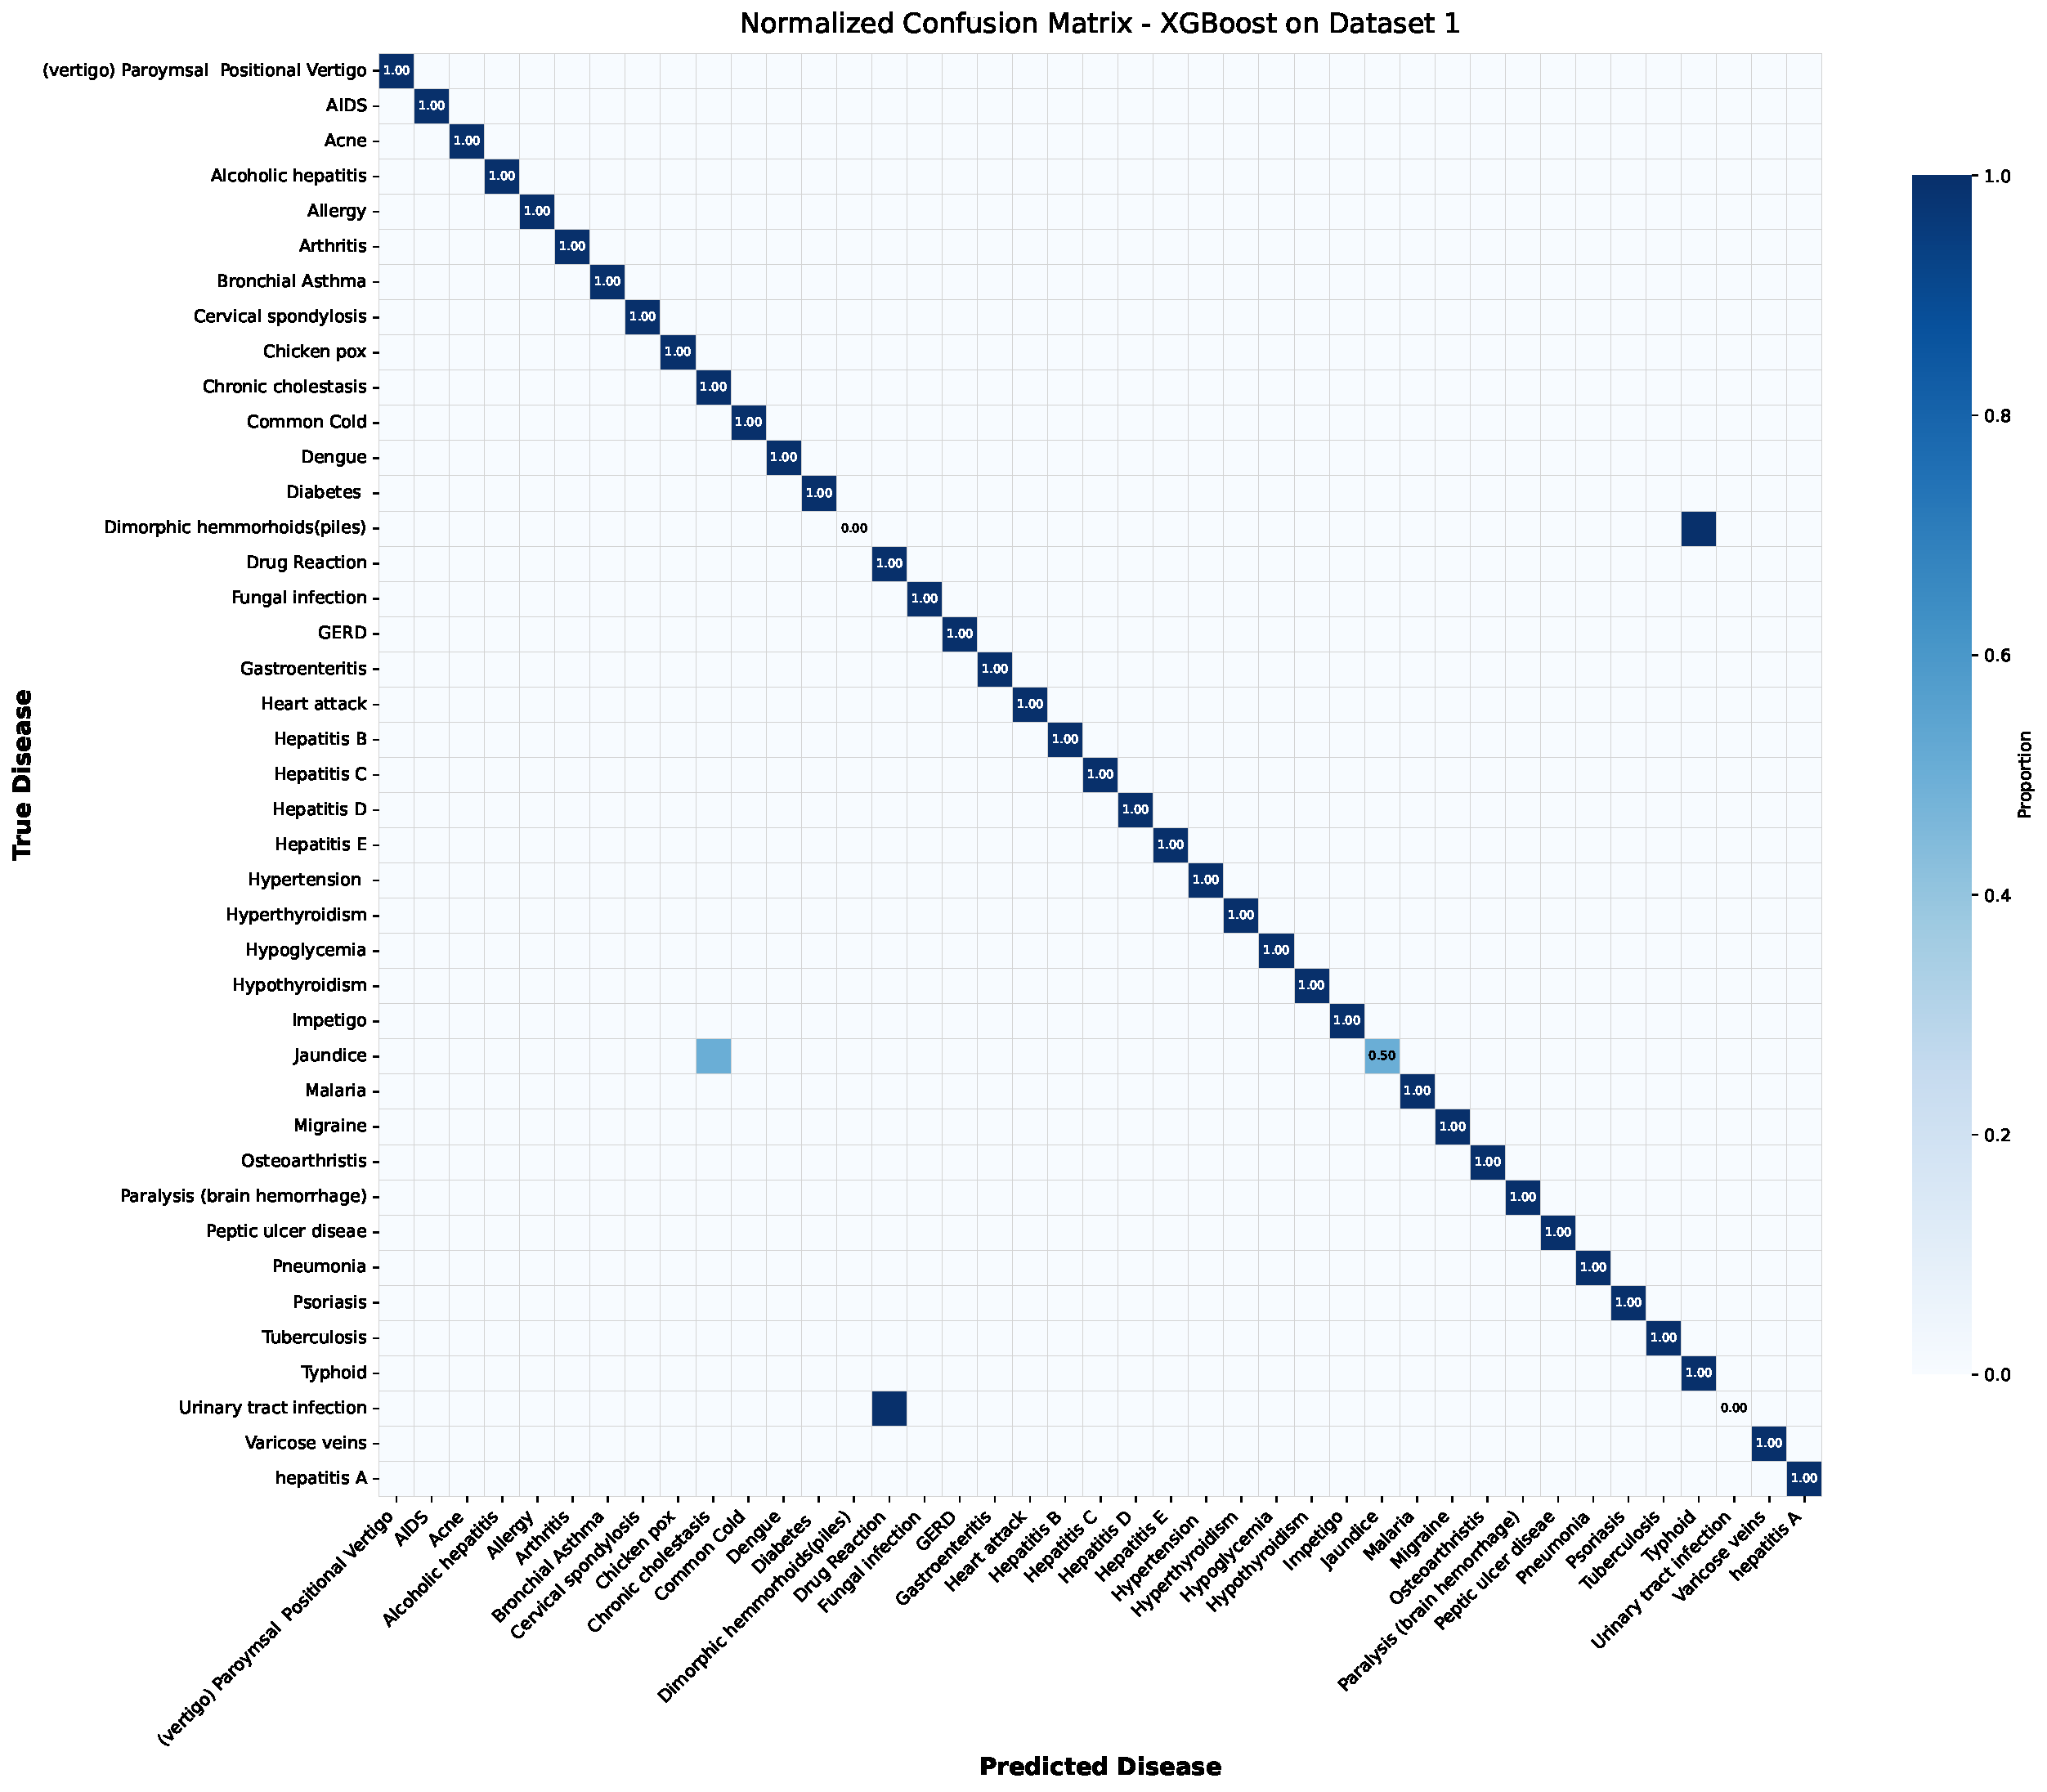
\includegraphics[width=0.85\textwidth]{figures/confusion_matrix.pdf}
\caption{Normalized confusion matrix for XGBoost on Dataset~1. Darker cells on the diagonal indicate correct classifications. Off-diagonal elements show misclassifications.}
\label{fig:confusion_matrix}
\end{figure}

The confusion matrix reveals that the majority of the errors are between diseases with similar symptoms. For instance, related respiratory diseases such as bronchitis and pneumonia were sometimes difficult to distinguish because of similar symptoms like cough, fever, and chest pain. Likewise, various types of skin problems were mixed up when they presented with a similar rash.

Interestingly, some of these confusion pairs are also clinically appropriate, as the diseases commonly have to be managed by the same specialist. A misclassification between two dermatological conditions would still direct the patient to a dermatologist, so the error would not affect the healthcare booking use case.

\section{Feature Importance Analysis}
\label{sec:feature_importance}

Random Forest and XGBoost can be used to calculate feature importances based on the contribution of each feature to the decision-making process. The top 15 most informative symptoms identified by XGBoost on Dataset~1 are shown in Figure~\ref{fig:feature_importance}.

\begin{figure}[H]
\centering
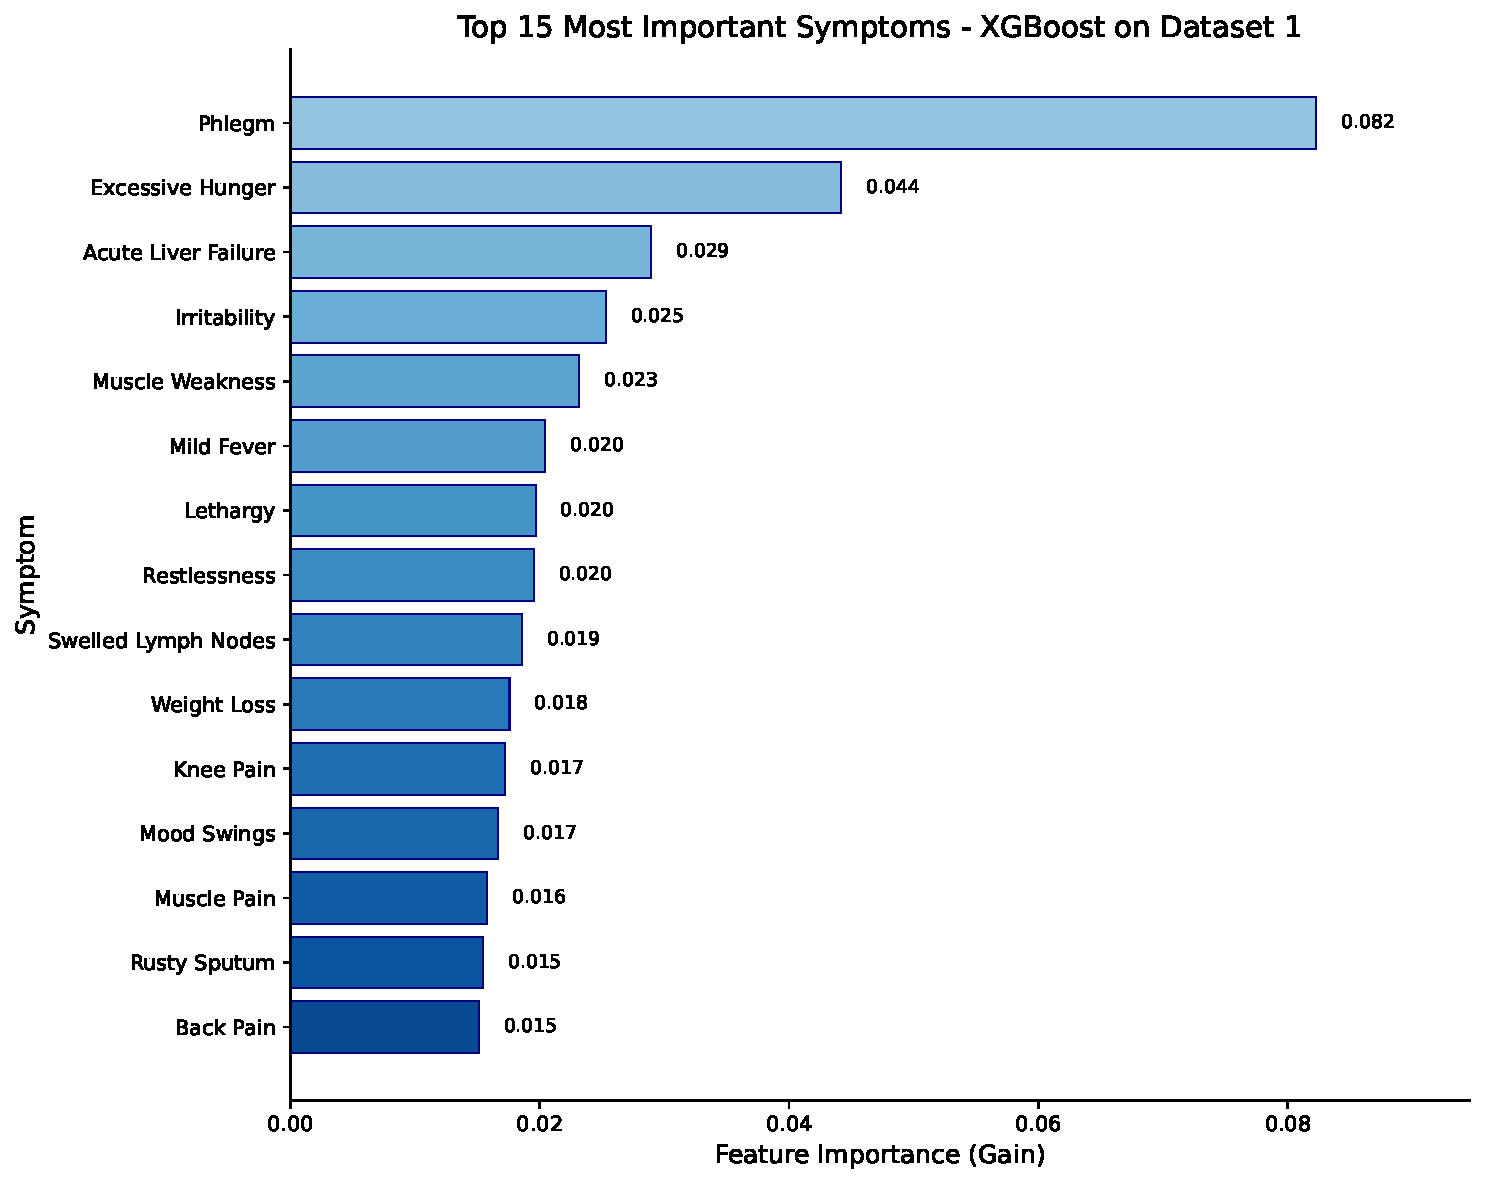
\includegraphics[width=0.85\textwidth]{figures/feature_importance.pdf}
\caption{Top 15 most important symptoms for XGBoost on Dataset~1, ranked by gain-based importance.}
\label{fig:feature_importance}
\end{figure}

The feature importance analysis revealed that certain symptoms provide more information than others. Disease-specific symptoms like ``skin\_rash'', ``chest\_pain'', and ``yellowish\_skin'' were high-ranking. Very general symptoms like fatigue and headache were not so important, as they are found in many diseases and give little discriminating signal.

This indicates that a short symptom questionnaire, consisting of only 15 or 20 carefully selected symptoms, could do as well and be much simpler for patients to complete. A discussion of this possibility is continued in Chapter~\ref{ch:conclusion}.
